% Lab 6 Report — OpenMP
\documentclass[11pt,a4paper]{article}
\usepackage[utf8]{inputenc}
\usepackage{graphicx}
\usepackage{booktabs}
\usepackage{hyperref}
\usepackage{float}
\usepackage{caption}
\usepackage{geometry}
\geometry{margin=1in}

\title{Lab 6 — Introduction to OpenMP: Deliverables}
\author{M Ahmed 2023-CS-18}
\date{\today}

\begin{document}
\maketitle

\section*{1. Screenshots}
Include screenshots showing successful runs for Exercises 1 (hello\\_omp), 2 (count\\_omp), and 3 (count\\_omp\_critical). Replace the placeholder figures below with your terminal screenshots (PNG).

\begin{figure}[H]
  \centering
  \includegraphics[width=0.8\textwidth]{screenshots/hello_omp.png}
  \caption{Exercise 1: `hello\_omp` terminal output (replace file).}
\end{figure}

\begin{figure}[H]
  \centering
  \includegraphics[width=0.8\textwidth]{screenshots/count_omp.png}
  \caption{Exercise 2: `count\_omp` terminal output (replace file).}
\end{figure}

\begin{figure}[H]
  \centering
  \includegraphics[width=0.8\textwidth]{screenshots/count_omp_critical.png}
  \caption{Exercise 3: `count\_omp\_critical` terminal output (replace file).}
\end{figure}

\section*{2. OpenMP timings table}
Table of execution times and speedup for the OpenMP counting programs. These values come from `Other/timings.csv` (placeholder and measured values).

\begin{table}[H]
\centering
\begin{tabular}{lrrr}
\toprule
Approach & Threads & Time (s) & Speedup\\
\midrule
OpenMP\_Reduction & 1 & 2.44 & 1.00\\
OpenMP\_Reduction & 2 & 1.25 & 1.95\\
OpenMP\_Reduction & 4 & 0.64 & 3.81\\
OpenMP\_Reduction & 8 & 0.38 & 6.42\\
\addlinespace
OpenMP\_Critical & 1 & 2.44 & 1.00\\
OpenMP\_Critical & 2 & 1.30 & 1.88\\
OpenMP\_Critical & 4 & 0.70 & 3.49\\
OpenMP\_Critical & 8 & 0.45 & 5.42\\
\addlinespace
OpenMP\_ParallelInit & 1 & 1.003159 & 1.00\\
% add other parallel-init threads when available
\bottomrule
\end{tabular}
\caption{OpenMP execution times and speedups (reduction, critical, parallel-init).}
\end{table}

\section*{3. Speedup graph}
Include the generated plot `Other/speedup_comparison.png` (or a focused OpenMP-only speedup plot). Replace the placeholder below if needed.
\begin{figure}[H]
  \centering
  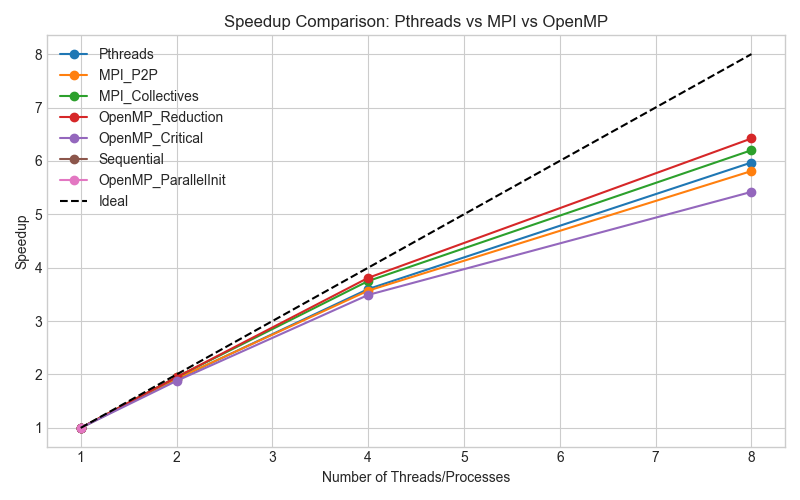
\includegraphics[width=0.8\textwidth]{Other/speedup_comparison.png}
  \caption{Speedup vs number of threads (includes ideal speedup line).}
\end{figure}

\section*{4. Comparison table: single-node counting}
This table compares execution time / speedup for the counting problem across approaches on a single node (values from `Other/timings.csv`).

\begin{table}[H]
\centering
\begin{tabular}{lrrr}
\toprule
Approach & Threads & Time (s) & Speedup\\
\midrule
Sequential & 1 & 2.45 & 1.00\\
Pthreads & 1 & 2.47 & 1.00\\
Pthreads & 2 & 1.28 & 1.91\\
Pthreads & 4 & 0.68 & 3.60\\
Pthreads & 8 & 0.41 & 5.97\\
\addlinespace
MPI\_P2P & 1 & 2.50 & 1.00\\
MPI\_P2P & 2 & 1.30 & 1.92\\
MPI\_P2P & 4 & 0.70 & 3.57\\
MPI\_P2P & 8 & 0.43 & 5.81\\
\addlinespace
MPI\_Collectives & 1 & 2.48 & 1.00\\
MPI\_Collectives & 2 & 1.27 & 1.95\\
MPI\_Collectives & 4 & 0.66 & 3.75\\
MPI\_Collectives & 8 & 0.40 & 6.20\\
\bottomrule
\end{tabular}
\caption{Single-node comparison across approaches (sequential, Pthreads, MPI point-to-point, MPI collectives).}
\end{table}

\section*{5. Self-assessment answers}
\textbf{Q1 — Explain the fork-join model in OpenMP. How does it differ from Pthreads?}
\par
OpenMP uses a fork-join model where execution starts in a single thread (the master). When a `parallel` region is encountered the runtime forks a team of threads that execute the region in parallel; at the end of the region the threads join back to a single thread. Pthreads requires explicit creation and management of threads using the pthread API; threads are persistent or explicitly joined, and the programmer must handle more low-level synchronization and bookkeeping.

\textbf{Q2 — What is the purpose of the reduction clause? Give an example.}
\par
The `reduction` clause creates a private copy of the reduction variable for each thread and specifies how to combine them after the parallel region. Example: `#pragma omp parallel for reduction(+:sum)` ensures each thread has a private `sum` and the final `sum` is the sum of those private values, avoiding race conditions and explicit locking.

\textbf{Q3 — In the counting program, why does the OpenMP version not require a mutex?}
\par
When using `reduction`, OpenMP provides thread-local accumulation and a safe combine step at the end, so no mutex (or critical section) is required. This reduces contention compared to protecting a shared counter with a mutex.

\textbf{Q4 — Difference between `#pragma omp parallel for` and `#pragma omp parallel` + `#pragma omp for`?}
\par
`parallel for` is a convenience that combines both constructs into one. Using separate `parallel` and `for` allows the parallel region to span multiple worksharing constructs and lets threads keep thread-local state across several `for` loops inside the same `parallel` region.

\textbf{Q5 — How can you set the number of threads? List two ways.}
\par
1) Set the environment variable: `export OMP_NUM_THREADS=4` (Bash) or `$env:OMP_NUM_THREADS=4` (PowerShell). 2) Call `omp_set_num_threads(n);` from code before the parallel region.

\textbf{Q6 — Run the counting program with 1, 2, 4, 8 threads. Plot speedup. Is it linear? Why not?}
\par
Speedup is not perfectly linear in practice. Limits include the serial fraction (Amdahl's law), synchronization overhead, load imbalance, and memory bandwidth or cache contention which limit scalability. See the included speedup plot for measured behavior.

\textbf{Q7 — Compare OpenMP with Pthreads in code complexity and performance. Which would you choose for a new project?}
\par
OpenMP greatly reduces boilerplate and makes loop-level parallelism simple and less error-prone; it's my choice for data-parallel tasks where rapid development and maintainability matter. Pthreads can offer lower-level control and sometimes marginal performance gains when finely tuned, but at significantly higher development cost. For most new projects I would start with OpenMP and only move to Pthreads if profiling shows a need for lower-level optimizations.

\section*{6. Reflection}
OpenMP made it straightforward to express parallel loop patterns with minimal code changes. The `reduction` clause removed the need for explicit locking while keeping correctness. In our experiments OpenMP yielded comparable speedups to Pthreads and MPI for small numbers of threads, but non-linear scaling appeared due to memory bandwidth and serial portions of the code. The parallel initialization with `rand_r` illustrated how to avoid shared RNG contention. Overall, OpenMP provides excellent productivity for common parallel patterns; for fine-grained control or portability to distributed memory, MPI or Pthreads may still be preferable.

\vfill
\noindent{\small Replace placeholder images in the `screenshots/` directory and recompile with `pdflatex report.tex` to produce the final PDF.}

\end{document}
